\documentclass[aspectratio=169]{beamer}

\usepackage{ccicons}
\usepackage{fontspec}
\usepackage{import}
\usepackage{listings}
\usepackage{tikz}

\subimport{../}{colors.tex}

\usetikzlibrary{
  arrows,
  arrows.meta,
  automata,
  backgrounds,
  calc,
  chains,
  decorations.pathreplacing,
  fit,
  matrix,
  overlay-beamer-styles,
  positioning,
  shapes,
  tikzmark,
}
\usetikzmarklibrary{listings}

\hypersetup{
  colorlinks=true,
  urlcolor=uclablue,
}

\setbeamercolor{frametitle}{fg=primarycolor}
\setbeamercolor{structure}{fg=primarycolor}
\setbeamercolor{enumerate item}{fg=black}
\setbeamercolor{itemize item}{fg=black}
\setbeamercolor{itemize subitem}{fg=black}

\setbeamersize{text margin left=26.6mm}
\addtolength{\headsep}{2mm}

\setbeamertemplate{navigation symbols}{}
\setbeamertemplate{headline}{}
\setbeamertemplate{footline}{}
\setbeamertemplate{itemize item}{\color{black}}
\setbeamertemplate{itemize items}[circle]

\setbeamertemplate{footline}{
  \begin{tikzpicture}[remember picture,
                      overlay,
                      shift={(current page.south west)}]
    \node [black!50, inner sep=2mm, anchor=south east]
          at (current page.south east) {\footnotesize \insertframenumber};
  \end{tikzpicture}
}

\setsansfont{Overpass}[Scale=MatchLowercase]
\setmonofont{Overpass Mono}[Scale=MatchLowercase]

\makeatletter
\newcommand\version[1]{\renewcommand\@version{#1}}
\newcommand\@version{}
\def\insertversion{\@version}

\newcommand\lecturenumber[1]{\renewcommand\@lecturenumber{#1}}
\newcommand\@lecturenumber{}
\def\insertlecturenumber{\@lecturenumber}
\makeatother

\setbeamertemplate{title page}
{
  \begin{tikzpicture}[remember picture,
                      overlay,
                      shift={(current page.south west)},
                      background rectangle/.style={fill=uclablue},
                      show background rectangle]
    \node [anchor=west, align=left, inner sep=0, text=white]
          (lecturenumber) at (\paperwidth / 6, \paperheight * 3 / 4)
          {\Large Lecture \insertlecturenumber};
    \node [inner sep=0, align=left, text=white, node distance=0,
           above left=of lecturenumber, anchor=south west, yshift=2mm]
          {\Large CS 111: Operating System Principles};
    \node (title) [inner sep=0, anchor=west, align=right, text=white]
          at (\paperwidth / 6, \paperheight / 2)
          {{\bfseries \Huge \inserttitle{}}};
    \node [inner sep=0, align=right, text=white, node distance=0,
           below right=of title, anchor=north east, yshift=-1mm]
          {{\footnotesize \ttfamily \insertversion}};
    \node [inner sep=0, text=white, align=left, anchor=west]
          (author) at (\paperwidth / 6, \paperheight / 4)
          {\insertauthor};
    \node [text=white, inner sep=0, align=left, node distance=0,
           below left=of author, anchor=north west, yshift=-2mm]
          {\insertdate};
    \node [align=right, anchor=south east, inner sep=2mm, text=white]
          (license) at (\paperwidth, 0)
          {\footnotesize This  work is licensed under a
           \href{http://creativecommons.org/licenses/by-sa/4.0/}
                {\color{uclagold} Creative Commons Attribution-ShareAlike 4.0
                 International License}};
    \node [text=white, inner sep=0, align=right, node distance=0,
           above right=of license, anchor=south east, xshift=-2mm]
          {\Large \ccbysa};
  \end{tikzpicture}
}

\tikzset{
  >=Straight Barb[],
  shorten >=1pt,
  initial text=,
}

\lstset{
  basicstyle=\footnotesize\ttfamily,
}


\lecturenumber{3}
\title{Libraries}
\version{2.0.1}
\author{Jon Eyolfson}
\date{June 29, 2021}

\begin{document}
  \begin{frame}[plain, noframenumbering]
    \titlepage
  \end{frame}

  \begin{frame}
    \frametitle{Applications May Pass Through Multiple Layers of Libraries}

    \begin{tikzpicture}[box/.style={draw, minimum width=3.5cm, minimum height=2em,
                                    inner sep=0.5em, node distance=0.5cm}]
      \draw [solarizedblue, dashed, thick] (0,0) -- ($(\textwidth - 3pt, 0)$);
      \node [solarizedblue, anchor=south east] at ($(\textwidth - 3pt, 0)$)
            (user) {User space};
      \node [solarizedblue, anchor=north east] at ($(\textwidth - 3pt, 0)$)
            (kernel) {Kernel space};

      \node [box, align=center, minimum width=9.2cm, xshift=-1cm] (libc) at ($(\textwidth/2 - 3pt, 1)$)
            {C Standard Library (libc)};

      \node [box, align=center, above=of libc, anchor=east, xshift=-0.1cm]
            {System Daemon (udev)};

      \node [box, align=center, above=of libc.north east, anchor=east, minimum width=4.5cm]
            (display) {Display Server (Wayland)};

      \node [box, above=of display.north east, anchor=east]
            {GUI Toolkit (GTK)};

      \node [box, fill=black!12.5,anchor=west] (app1) at (0, 5) {Lab 1};

      \node [box, fill=black!12.5, right=of app1] (app2) {NetworkManager};

      \node [box, fill=black!12.5, right=of app2] {Firefox};
    \end{tikzpicture}
  \end{frame}

  \begin{frame}
    \frametitle{C ABI, or Calling Convention for x86-64}

    System calls use registers, while C is stack based:
    \begin{itemize}
      \item Arguments pushed on the stack from right-to-left order
      \item \texttt{rax}, \texttt{rcx}, \texttt{rdx} are caller saved
      \item Remaining registers are callee saved
    \end{itemize}

    \vspace{4em}

    What advantages does this give us vs system call ABI? Disadvantages?
  \end{frame}

  \begin{frame}
    \frametitle{System Calls are Rare in C}

    Mostly you'll be using functions from the C standard library instead

    \vspace{2em}

    Most system calls have corresponding function calls in C, but may:
    \begin{itemize}
      \item Set \texttt{errno}
      \item Buffer reads and writes (reduce the number of system calls)
      \item Simplify interfaces (function combines two system calls)
      \item Add new features
    \end{itemize}
  \end{frame}

  \begin{frame}[fragile]
    \frametitle{C \texttt{exit} Has Additional Features}

    System call \texttt{exit} (or \texttt{exit\_group}): the program
    stops at that point

    \vspace{1em}

    C \texttt{exit}: there's a feature to register functions to call
    on program exit (\texttt{atexit})

    \vspace{1em}

    \begin{lstlisting}[xleftmargin=2em]
#include <stdio.h>
#include <stdlib.h>

void fini(void) {
  puts("Do fini");
}

int main(int argc, char **argv) {
  atexit(fini);
  puts("Do main");
  return 0;
}
    \end{lstlisting}
    \vspace{-1em}
    \begin{flushright}
      \lstinline|examples/lecture-03/atexit-example|
    \end{flushright}
  \end{frame}

  \begin{frame}
    \frametitle{Normal Compilation in C}

    \begin{center}
    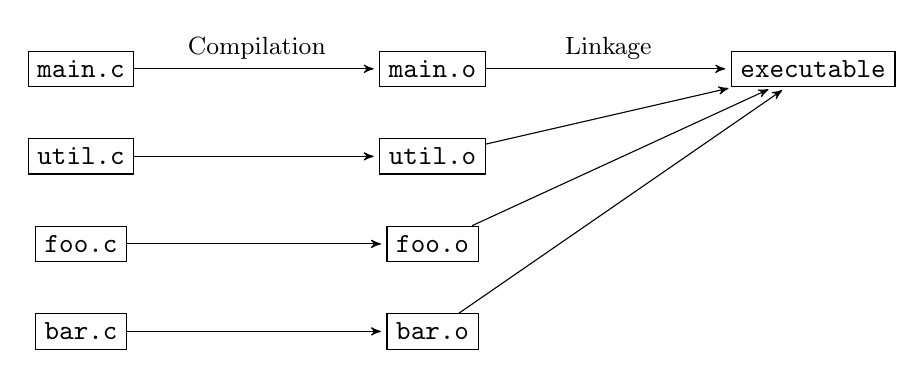
\begin{tikzpicture}[>=stealth', shorten >=2pt]
      \node[draw, align=left] (main) {\texttt{main.c}};
      \node[draw, align=left, below=of main, yshift=1em] (util)
           {\texttt{util.c}};
      \node[draw, align=left, below=of util, yshift=1em] (foo)
           {\texttt{foo.c}};
      \node[draw, align=left, below=of foo, yshift=1em] (bar)
           {\texttt{bar.c}};

      \node[draw, align=left, right=of main, xshift=6em] (main-obj)
           {\texttt{main.o}};
      \node[draw, align=left, below=of main-obj, yshift=1em] (util-obj)
           {\texttt{util.o}};
      \node[draw, align=left, below=of util-obj, yshift=1em] (foo-obj)
           {\texttt{foo.o}};
      \node[draw, align=left, below=of foo-obj, yshift=1em] (bar-obj)
           {\texttt{bar.o}};

      \node[draw, align=left, right=of main-obj, xshift=6em] (exec)
           {\texttt{executable}};

      \draw[->] (main) -- node [above] {\small Compilation} (main-obj);
      \draw[->] (util) -- (util-obj);
      \draw[->] (foo) -- (foo-obj);
      \draw[->] (bar) -- (bar-obj);
      \draw[->] (main-obj) -- node [above] {\small Linkage} (exec);
      \draw[->] (util-obj) -- (exec);
      \draw[->] (foo-obj) -- (exec);
      \draw[->] (bar-obj) -- (exec);
    \end{tikzpicture}
    \end{center}

    \vspace{1em}

    Note: object files (\texttt{.o}) are just ELF files with code for functions
  \end{frame}

  \begin{frame}
    \frametitle{Static Libraries Are Included At Link Time}
    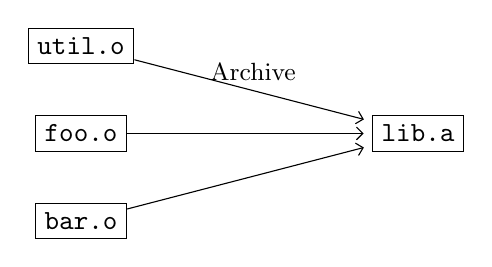
\begin{tikzpicture}[shorten >=3pt]
      \node[draw, align=left] (util-obj)
           {\texttt{util.o}};
      \node[draw, align=left, below=of util-obj, yshift=1em] (foo-obj)
           {\texttt{foo.o}};
      \node[draw, align=left, below=of foo-obj, yshift=1em] (bar-obj)
           {\texttt{bar.o}};

      \node[draw, align=left, right=of foo-obj, xshift=6em] (static)
           {\texttt{lib.a}};

      \draw[->] (util-obj) -- node [above] {\small Archive} (static);
      \draw[->] (foo-obj) -- (static);
      \draw[->] (bar-obj) -- (static);
    \end{tikzpicture}

    \begin{flushright}
    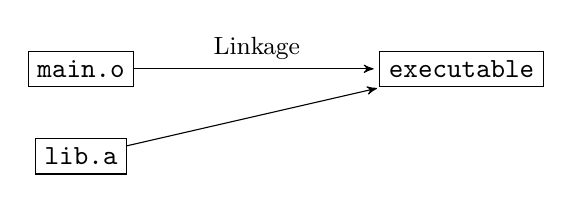
\begin{tikzpicture}[>=stealth', shorten >=2pt]

      \node[draw, align=left] (main-obj)
           {\texttt{main.o}};
      \node[draw, align=left, below=of main-obj, yshift=1em] (static)
           {\texttt{lib.a}};

      \node[draw, align=left, right=of main-obj, xshift=6em] (exec)
           {\texttt{executable}};

      \draw[->] (main-obj) -- node [above] {\small Linkage} (exec);
      \draw[->] (static) -- (exec);
    \end{tikzpicture}
    \end{flushright}
  \end{frame}

  \begin{frame}
    \frametitle{Dynamic Libraries Are For Reusable Code}

    The C standard library is a dynamic library (\texttt{.so}), like any other
    on the system

    \hspace{1em} Basically a collection of \texttt{.o} files containing function
    definitions

    \vspace{1em}

    Multiple applications can use the same library:

    \vspace{1em}

    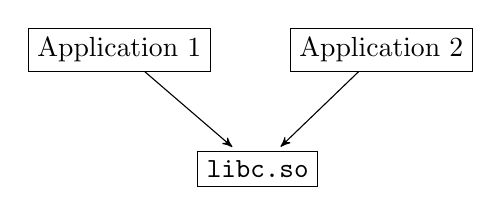
\begin{tikzpicture}[>=stealth', shorten >=2pt]
      \node[draw] (app1) {Application 1};
      \node[draw, right=of app1] (app2) {Application 2};
      \node[draw, below=of app1, xshift=5em] (libc) {\texttt{libc.so}};
      \draw[->] (app1) -- (libc);
      \draw[->] (app2) -- (libc);
    \end{tikzpicture}

    \vspace{1em}

    The operating system only loads \texttt{libc.so} in memory once, and shares
    it

    \hspace{1em} The same physical page corresponds to different virtual pages
    in processes
  \end{frame}

  \begin{frame}
    \frametitle{Dynamic Libraries Are Included At Runtime}

    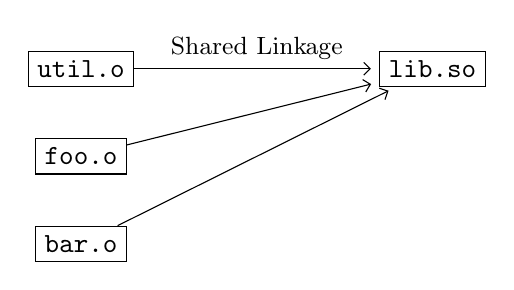
\begin{tikzpicture}[shorten >=3pt]
      \node[draw, align=left] (util-obj)
           {\texttt{util.o}};
      \node[draw, align=left, below=of util-obj, yshift=1em] (foo-obj)
           {\texttt{foo.o}};
      \node[draw, align=left, below=of foo-obj, yshift=1em] (bar-obj)
           {\texttt{bar.o}};

      \node[draw, align=left, right=of util-obj, xshift=6em] (dynamic)
           {\texttt{lib.so}};

      \draw[->] (util-obj) -- node [above] {\small Shared Linkage} (dynamic);
      \draw[->] (foo-obj) -- (dynamic);
      \draw[->] (bar-obj) -- (dynamic);
    \end{tikzpicture}

    \begin{flushright}
    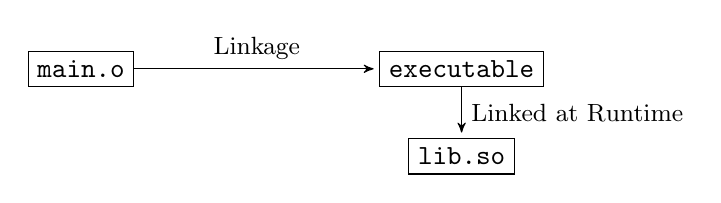
\begin{tikzpicture}[>=stealth', shorten >=2pt]

      \node[draw, align=left] (main-obj)
           {\texttt{main.o}};

      \node[draw, align=left, right=of main-obj, xshift=6em] (exec)
           {\texttt{executable}};

      \node[draw, align=left, below=of exec, yshift=1em] (dynamic)
           {\texttt{lib.so}};

      \draw[->] (main-obj) -- node [above] {\small Linkage} (exec);
      \draw[->] (exec) -- node [right] {\small Linked at Runtime} (dynamic);
    \end{tikzpicture}
    \end{flushright}
  \end{frame}

  \begin{frame}
    \frametitle{Useful Command Line Utilities for Dynamic Libraries}

    \texttt{ldd <executable>}

    \hspace{1em} shows which dynamic libraries an executable uses

    \vspace{4em}

    \texttt{objdump -T <library>}

    \hspace{1em} shows the symbols (often just function names) that are in the
    library

    \vspace{1em}

    You can also use \texttt{objdump -d} to disassemble the library
  \end{frame}

  \begin{frame}
    \frametitle{Static vs Dynamic Libraries}

    Another option is to statically link your code

    \hspace{1em} Basically copies the \texttt{.o} files directly into the
    executable

    \vspace{2em}

    The drawbacks compared to dynamic libraries:
    \begin{itemize}
      \item Statically linking prevents re-using libraries, commonly used
            libraries have many duplicates
      \item Any updates to a static library requires the executable to be
            recompiled
    \end{itemize}

    \vspace{2em}

    What are issues with dynamic libraries?
  \end{frame}

  \begin{frame}
    \frametitle{Dynamic Libraries Updates Can Break Executables with ABI
                Changes}

    An update to a dynamic library can easily cause an executable using it to
    crash

    \vspace{1em}

    Consider the following in a dynamic library:

    \hspace{1em} A \texttt{struct} with multiple fields corresponding to
    a specific data layout (C ABI)

    \vspace{1em}

    \structure{An executable accesses the fields of the \texttt{struct} in the
               dynamic library}

    \vspace{1em}

    Now if the dynamic libraries reorders the fields

    \hspace{1em} The executable uses the old offsets and is now wrong

    \vspace{1em}

    Note: this is OK if the dynamic library never exposes the fields of a
    \texttt{struct}
  \end{frame}

  \begin{frame}[fragile]
    \frametitle{C Uses a Consistent ABI for \texttt{struct}s}

    \texttt{struct}s are laid out in memory with the fields matching the
    declaration order

    \hspace{2em} C compilers ensure the ABI of \texttt{struct}s are the
    consistent for an architecture

    \vspace{2em}

    Consider the following structures:

    \vspace{1em}

    \begin{columns}
      \begin{column}{0.4\textwidth}
        Library v1:
        \begin{lstlisting}[basicstyle=\small\ttfamily]
struct point {
  int y;
  int x;
};
        \end{lstlisting}
      \end{column}
      \begin{column}{0.4\textwidth}
        Library v2:
        \begin{lstlisting}[basicstyle=\small\ttfamily]
struct point {
  int x;
  int y;
};
        \end{lstlisting}
      \end{column}
    \end{columns}

    \vspace{1em}

    For v1 the \texttt{x} field is offset by 4 bytes from the start of
    \texttt{struct point}'s base

    \hspace{2em} For v2 it is offset by 0 bytes, and this difference
    will cause problems
  \end{frame}

  \begin{frame}[fragile]
    \frametitle{ABI Stable Code Should Always Print ``1, 2''}

    \begin{lstlisting}[basicstyle=\small\ttfamily]
int main(int argc, char **argv) {
  struct point *p = point_create(1, 2);

  printf("point (x, y) = %d, %d (using library)\n",
         point_get_x(p), point_get_y(p));

  struct point_v1 *p_v1 = (struct point_v1 *) p;
  printf("point (x, y) = %d, %d (using v1)\n", p_v1->x, p_v1->y);

  struct point_v2 *p_v2 = (struct point_v2 *) p;
  printf("point (x, y) = %d, %d (using v2)\n", p_v2->x, p_v2->y);

  point_destroy(p);
  return 0;
}
    \end{lstlisting}

  \end{frame}

  \begin{frame}[fragile]
    \frametitle{Mismatched Versions of This Library Causes Unexpected Results}

    The definition of \texttt{struct point} in both libraries is different

    \hspace{2em} Order of \texttt{x} and \texttt{y} change (and therefore their offsets)

    \vspace{2em}

    Our code works correctly with either v1 or v2 of the library

    \hspace{2em} The stable ABI is in \lstinline|libpoint.h| (it hides the \texttt{struct})

    \hspace{4em} If you expose a \texttt{struct} it becomes part of your ABI!

    \vspace{2em}

    If the \texttt{struct point} was exposed we get unexpected results with v2

    \hspace{2em} This would be compiled into your program if the \texttt{struct}
    was visible!
  \end{frame}

  \begin{frame}[fragile]
    \frametitle{Try the Previous Example}

    It's in \lstinline|examples/lecture-03| directory

    \vspace{2em}

    Set \texttt{LD\_LIBRARY\_PATH} to \lstinline|lib-v1| or \lstinline|lib-v2|
    to  simulate a library update

    \vspace{2em}

    Run the following commands to see for yourself:
    \begin{lstlisting}[commentstyle={}, xleftmargin=2em]
LD_LIBRARY_PATH=lib-v1 ./point-example
LD_LIBRARY_PATH=lib-v2 ./point-example
    \end{lstlisting}

    \vspace{2em}

    Note: you'd also have a problem if you compiled with v2 and used v1
  \end{frame}

  \begin{frame}
    \frametitle{Semantic Versioning Meets Developer's Expectations}

    From \url{https://semver.org/}, given a version number MAJOR.MINOR.PATCH,
    increment the:

    \begin{itemize}
      \item MAJOR version when you make incompatible API\structure{/ABI} changes
      \item MINOR version when you add functionality in a backwards-compatible
            manner
      \item PATCH version when you make backwards-compatible bug fixes
    \end{itemize}
  \end{frame}

  \begin{frame}[fragile]
    \frametitle{Dynamic Libraries Allow Easier Debugging}

    Control dynamic linking with environment variables

    \hspace{2em} \texttt{LD\_LIBRARY\_PATH} and \texttt{LD\_PRELOAD}

    \vspace{2em}

    Consider the following example:
    \begin{lstlisting}[xleftmargin=2em]
#include <stdlib.h>
#include <stdio.h>

int main(int argc, char **argv)
{
  int *x = malloc(sizeof(int));
  printf("x = %p\n", x);
  free(x);
  return 0;
}
    \end{lstlisting}
  \end{frame}

  \begin{frame}[fragile]
    \frametitle{We Can Monitor All Allocations with Our Own Library}

    Normal runs of \texttt{alloc-example} outputs:
    \begin{lstlisting}
x = 0x561116384260
    \end{lstlisting}

    \vspace{1em}

    Create \texttt{alloc-wrapper.so} that outputs all \texttt{malloc} and
    \texttt{free} calls

    \vspace{1em}

    Run: \lstinline|LD_PRELOAD=./alloc-wrapper.so  ./alloc-example|

    \begin{lstlisting}[xleftmargin=2em]
Call to malloc(4) = 0x55c12aa40260                  
Call to malloc(1024) = 0x55c12aa40280
x = 0x55c12aa40260
Call to free(0x55c12aa40260)
    \end{lstlisting}

    \vspace{1em}

    Interesting, we did not make 2 \texttt{malloc} calls
  \end{frame}

  \begin{frame}
    \frametitle{Detecting Memory Leaks}

    \texttt{valgrind} is another useful tool to detect memory leaks from
    \texttt{malloc} and \texttt{free}

    \hspace{1em} Usage: \texttt{valgrind <executable>}

    \vspace{2em}

    Here's a note from the \texttt{man} pages regarding what we saw:

    \vspace{1em}

    ``The GNU C library (\texttt{libc.so}), which is used by all programs,
      may allocate memory for its own uses. Usually it doesn't bother to free
      that memory when the program ends—there would be no point, since the Linux
      kernel reclaims all process resources when a process exits anyway, so it
      would just slow things down.''

    \vspace{2em}

    \structure{Note: this does not excuse you from not calling \texttt{free}!}
  \end{frame}

  \begin{frame}
    \frametitle{Standard File Descriptors for Unix}

    All command line executables use the following standard for file
    descriptors:

    \begin{itemize}
      \item \texttt{0} --- \texttt{stdin} (Standard input)
      \item \texttt{1} --- \texttt{stdout} (Standard output)
      \item \texttt{2} --- \texttt{stderr} (Standard error)
    \end{itemize}

    \vspace{2em}

    The terminal emulators job is to:
    \begin{itemize}
      \item Translate key presses to bytes and write to \texttt{stdin}
      \item Display bytes read from \texttt{stdout} and \texttt{stderr}
      \item May redirect file descriptors between processes
    \end{itemize}
  \end{frame}

  \begin{frame}[fragile]
    \frametitle{Checking Open File Descriptors on Linux}

    \texttt{/proc/<PID>/fd} \hspace{0.5em} is a directory containing all open
    file descriptors for a process

    \texttt{ps x} \hspace{0.5em} command shows a list of processes matching your
    user (lots of other flags)

    \vspace{1em}

    A terminal emulator may give the output:
    \begin{lstlisting}[basicstyle=\small\ttfamily]
> ls -l /proc/21151/fd
0 -> /dev/tty1
1 -> /dev/tty1
2 -> /dev/tty1
    \end{lstlisting}

    \vspace{2em}

    \texttt{lsof <file>} \hspace{0.5em} shows you what processes have the file
    open

    \hspace{2em} For example, processes using C: \hspace{0.5em}
    \texttt{lsof /lib/libc.so.6}
  \end{frame}

  \begin{frame}
    \frametitle{Operating Systems Provide the Foundation for Libraries}

    We learned:
    \begin{itemize}
      \item Dynamic libraries and a comparison to static libraries
      \begin{itemize}
        \item How to manipulate the dynamic loader
      \end{itemize}
      \item Example of issues from ABI changes without API changes
      \item Standard file descriptor conventions for UNIX
    \end{itemize}
  \end{frame}

\end{document}
